\documentclass[main.tex]{subfiles}

\begin{document}

\section{Software Architecture}\label{sec:software_architecture}

\subsection{Deployment Diagram}

The deployment diagram provides an overview of the distribution and interaction of the components within our decentralized application (dApp). 
This visual representation is crucial for understanding how the different parts of the system connect and collaborate to deliver a functional and cohesive application.\\

\begin{figure}[htbp] % Posizionamento dell'immagine
    \centering % Centra l'immagine orizzontalmente
    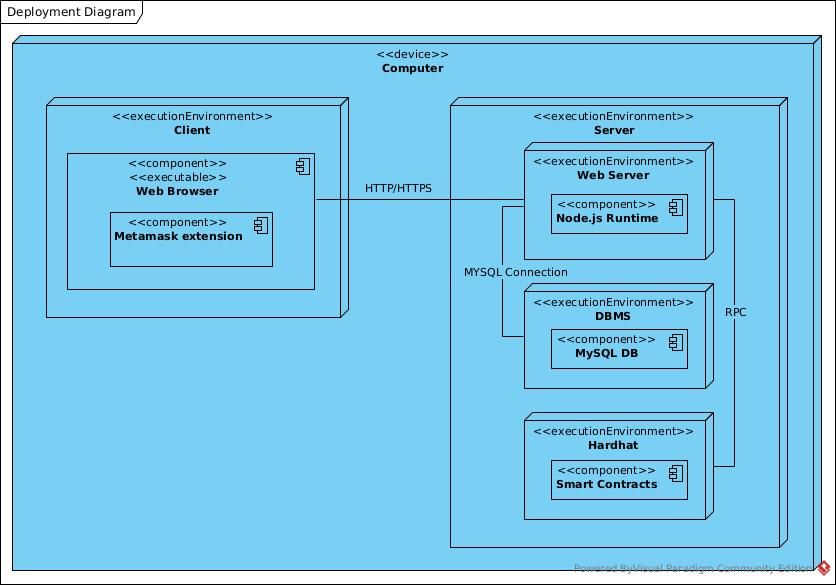
\includegraphics[width=1\textwidth]{src/diagrams/Deployment Diagram.jpg} % Imposta la larghezza dell'immagine al 50% della larghezza del testo
    \caption{dApp Deployment Diagram} % Didascalia dell'immagine
    \label{fig:deployDiag} % Etichetta per i riferimenti incrociati
\end{figure}

Our dApp is designed as a web application using JavaScript and Handlebars (hbs). Users interact with the dApp through this web interface, which is supported by client 
libraries such as Web3.js or Ethers.js for blockchain interactions and MetaMask for transaction management.\\

The blockchain management is facilitated by smart contracts deployed on the Ethereum network. These smart contracts handle the management of tokens (DNT), processing 
of NFT transactions, and recording of game scores. Hardhat, a development environment for Ethereum, is utilized for deploying and testing these smart contracts.\\

Hardhat streamlines the development process by providing local blockchain environments, debugging tools, and integration with the Ethereum network.\\

MetaMask, a browser extension wallet, allows users to connect their Ethereum wallets to the dApp securely. It provides a user-friendly interface for managing private 
keys and interacting with smart contracts on the Ethereum network.\\

The backend includes a Node.js API server and a MySQL database, managed via phpMyAdmin, to store essential data such as wallet-username associations and game scores. 
All components are hosted on cloud platforms, ensuring both scalability and availability.\\

This diagram offers a clear depiction of the connections and dependencies among these elements, aiding in the understanding of the architecture and supporting 
effective system management throughout the development and production phases.

\subsection{Use Case Diagram}
The use case diagram outlines key blockchain-driven interactions within the dApp, such as connecting the wallet via MetaMask, registering, participating in mini-games
 to earn tokens (DNT) by placing in the top three, and completing quizzes for token rewards. It also includes token transactions for buying and selling, all securely 
 facilitated through smart contracts.

 \begin{figure}[htbp] % Posizionamento dell'immagine
    \centering % Centra l'immagine orizzontalmente
    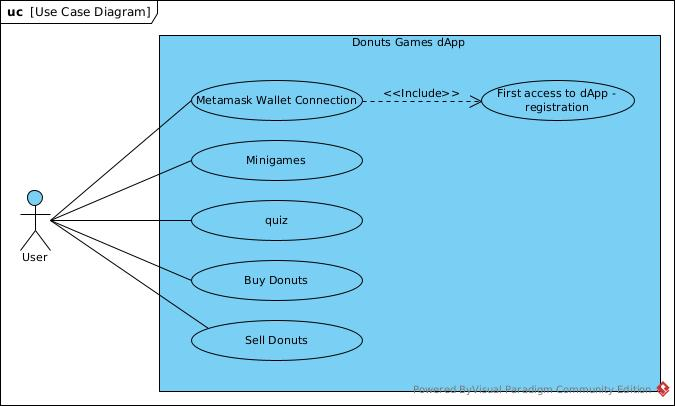
\includegraphics[width=1\textwidth]{src/diagrams/Use Case Diagram.jpg} % Imposta la larghezza dell'immagine al 50% della larghezza del testo
    \caption{dApp Use Case Diagram} % Didascalia dell'immagine
    \label{fig:useCaseDiag} % Etichetta per i riferimenti incrociati
\end{figure}
%Metamask wallet connection + First wallet connection - registration.jpg
\begin{figure}[htbp] % Posizionamento dell'immagine
    \centering % Centra l'immagine orizzontalmente
    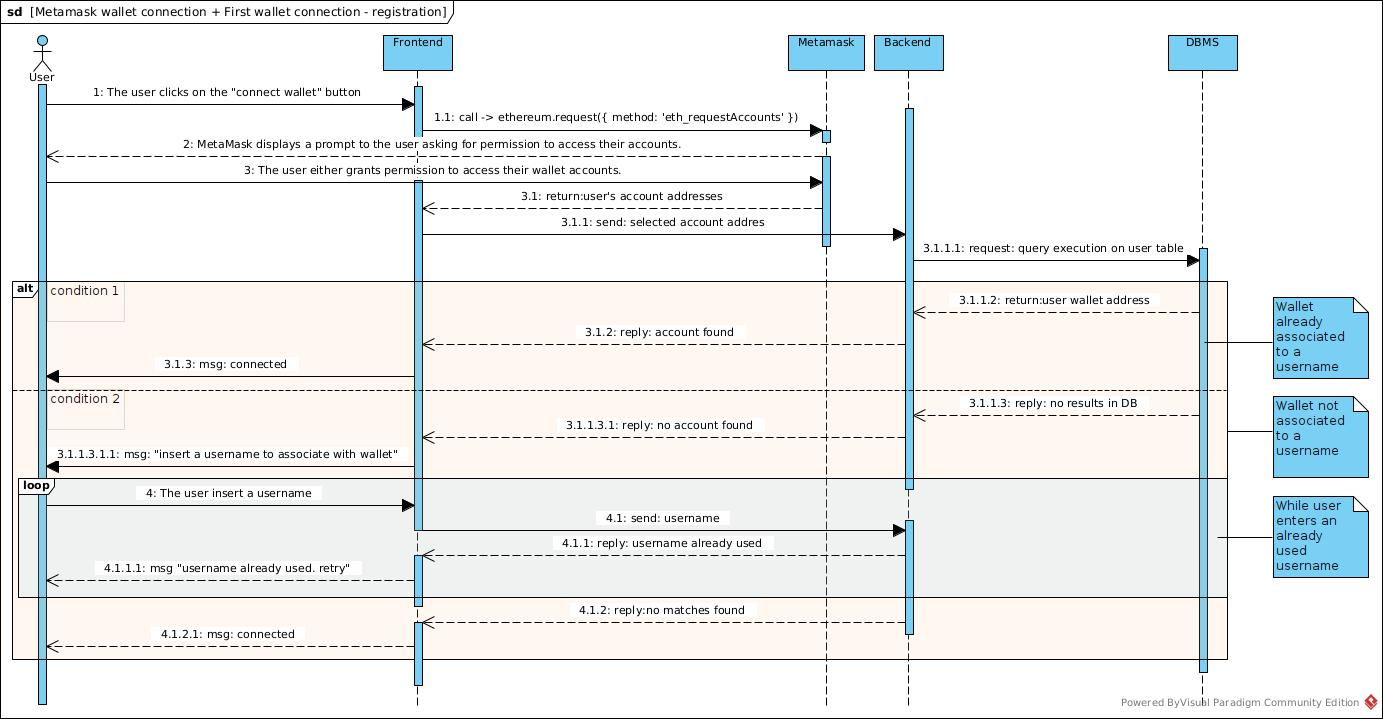
\includegraphics[width=1\textwidth]{src/diagrams/Metamask wallet connection + First wallet connection - registration.jpg} % Imposta la larghezza dell'immagine al 50% della larghezza del testo
    \caption{Wallet connection sequence diagram} % Didascalia dell'immagine
    \label{fig:WalletConnect_seqDiag} % Etichetta per i riferimenti incrociati
\end{figure}
\end{document}